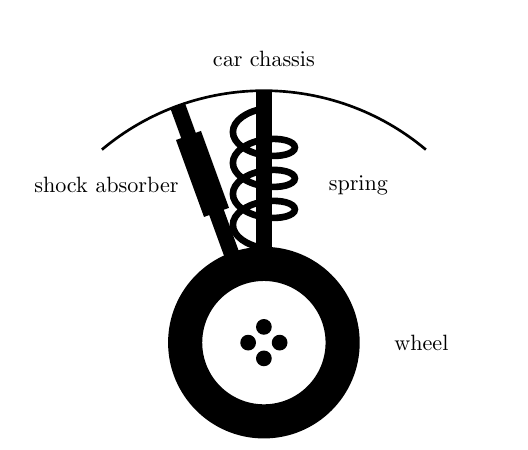
\begin{tikzpicture}[scale=1,inner sep=0pt,outer sep=0pt,very thick]

\useasboundingbox (-3,-1) rectangle (3,4); 
\begin{scope}[transform canvas={scale=.8}]
\draw[line width=3pt,decorate,decoration={coil,segment length=14,amplitude=14}] (0,1.5) -- (0,4);
\draw[line width=7pt] (0,0) -- (0,4);
\draw (1.5,2.5) node {spring};

\draw[line width=7pt,rotate=20] (0,0) -- (0,4);
\draw[line width=12pt,rotate=20] (0,2.2) -- (0,3.5);
\draw (-2.5,2.5) node {shock absorber};

\draw (0,0) node[draw,fill=black,circle,minimum width=3cm] {};
\draw (0,0) node[draw,fill=white,circle,minimum width=2cm] {};
\draw (.25,0) node[fill=black,circle,minimum width=.25cm] {};
\draw[rotate=90] (.25,0) node[fill=black,circle,minimum width=.25cm] {};
\draw[rotate=180] (.25,0) node[fill=black,circle,minimum width=.25cm] {};
\draw[rotate=-90] (.25,0) node[fill=black,circle,minimum width=.25cm] {};
\draw (2.5,0) node {wheel};

\draw (50:4) arc (50:130:4);
\draw (0,4.5) node {car chassis};
\end{scope}
\end{tikzpicture}
